\documentclass[12pt,a4paper]{article}
\usepackage[latin1]{inputenc}
\usepackage[spanish]{babel}
\usepackage{amsmath}
\usepackage{amsfonts}
\usepackage{amssymb}
\usepackage{graphicx}
\usepackage[usenames]{color}
\usepackage{xcolor}
\usepackage[spanish, onelanguage, linesnumbered,lined,boxed,commentsnumbered]{algorithm2e}

% Default fixed font does not support bold face
\DeclareFixedFont{\ttb}{T1}{txtt}{bx}{n}{12} % for bold
\DeclareFixedFont{\ttm}{T1}{txtt}{m}{n}{12}  % for normal
% Custom colors
\usepackage{color}
\definecolor{deepblue}{rgb}{0,0,0.5}
\definecolor{deepred}{rgb}{0.6,0,0}
\definecolor{deepgreen}{rgb}{0,0.5,0}

\usepackage{listings}

% Python style for highlighting
\newcommand\pythonstyle{\lstset{
language=Python,
basicstyle=\ttm,
otherkeywords={self},             % Add keywords here
keywordstyle=\ttb\color{deepblue},
emph={MyClass,__init__},          % Custom highlighting
emphstyle=\ttb\color{deepred},    % Custom highlighting style
stringstyle=\color{deepgreen},
frame=tb,                         % Any extra options here
showstringspaces=false            % 
}}


% Python environment
\lstnewenvironment{python}[1][]
{
\pythonstyle
\lstset{#1}
}
{}

% Python for external files
\newcommand\pythonexternal[2][]{{
\pythonstyle
\lstinputlisting[#1]{#2}}}

% Python for inline
\newcommand\pythoninline[1]{{\pythonstyle\lstinline!#1!}}

\usepackage[left=2cm,right=2cm,top=2cm,bottom=2cm]{geometry}


\author{
	%\texttt{Legends}
}
\date{
27 de Noviembre del 2017
}
\title{An\'alisis de la implementaci\'on del algoritmo para n\'umeros primos}

\begin{document}
\maketitle
\begin{center}
Equipo 2:
\end{center}
\begin{align*}
	&\textrm{Maria Luisa Borrego.} 					\qquad &(1837482)\\
	&\textrm{Rafael Enrique Almaraz.}				\qquad &(1579795)\\
	&\textrm{Artemio Guajardo.} 					\qquad &(1590417)\\
	&\textrm{Ana Cecilia Garc\'ia.}					\qquad &(1749760)\\
	&\textrm{Hayde\'e Judith Arriaga.}				\qquad &(1659539)\\
	&\textrm{Jos\'e Manuel Tapia.}					\qquad &(1729372)
\end{align*}


%Este es un comentario que no se ve en el pdf jejeje xdXDxd
Sabemos que en matem\'aticas, un n\'umero primo es un n\'umero natural mayor que 1 que tiene \'unicamente dos divisores distintos: \'el mismo y el 1. Por el contrario, los n\'umeros compuestos son los n\'umeros naturales que tienen alg\'un divisor natural aparte de s\'i mismos y del 1, por lo tanto, pueden factorizarse. El n\'umero 1, por convenio, no se considera ni primo ni compuesto. Anteriormente se trabaj\'o con el algoritmo para obtener n\'umeros primos, en esta ocasi\'on toca analizar los resultados de \'esta implementaci\'on aplicando ciertas restricciones con el fin de observar la complejidad de las operaciones realizadas seg\'un sea la restricci\'on.

\section{Implementaci\'on del algoritmo}



Como se mencion\'o en la introducci\'on, las condiciones para que un n\'umero sea primo son que sea mayor a 1 y que sea \'unicamente divisible entre 1 y \'el mismo, pero adem\'as se conoce una propiedad que dice que si un n\'umero no tiene divisores menores o iguales que su ra\'iz cuadrada, entonces es un n\'umero primo. Estas condiciones fueron tomadas en cuenta para implementar el algoritmo, obteniendo una complejidad de $\mathcal{O}(\sqrt{n})$, donde $n$ es el n\'umero que se busca saber si es primo o no.

La implementaci\'on del algoritmo es la siguiente:
\begin{python}
def itsPrime(n):
    if n<=1:
        return False
    m=2
    while m*m<=n:
        if n%m==0:
            return False
        m+=1
    return True
\end{python}

Para fines del proyecto, de igual forma se implemento una variante de la funci\'on anterior, que en vez de retornar si un n\'umero es primo o no, regresa la cantidad de operaciones necesarias para determinar si cierto n\'umero $n$ es primo o no. 

\begin{python}
def esPrimo(n):
    cnt=0
    if n<=1:
        return cnt
    m=2
    while m*m<=n:
        cnt+=1
        if n%m==0:
            return cnt
        m+=1
    return cnt
\end{python}

Para realizar las gr\'aficas de la siguiente secci\'on, se uso la siguiente funci\'on que recibe los valores que se tienen para cada uno de los ejes, el nombre y el t\'itulo de dicha gr\'afica. 
\begin{python}
def graficar(xs,ys,imagen,titulo):
    x=np.linspace(1,100000)
    plt.plot(x,x**(0.5),label="Raiz de n",color="green")
    plt.plot(xs,ys, label=titulo)
    plt.xlabel("Numero")
    plt.ylabel("Cantidad de operaciones")
    plt.title(titulo) 
    plt.legend()
    plt.savefig(imagen)
    plt.show()
\end{python}
En donde, para llamar a dicha funci\'on se realizaron los siguientes prec\'alculos:
\begin{python}
G1xs=range(1,100001,251)
G1ys=[esPrimo(x) for x in G1xs]
G2xs=range(1,50001,251)
G2ys=[esPrimo(x) for x in G2xs]
G3xs=range(50000,100001,251)
G3ys=[esPrimo(x) for x in G3xs]
G4xs=[x for x in range(1,100001,251) if x%2==0]
G4ys=[esPrimo(x) for x in G4xs]
G5xs=[x for x in range(1,100001,251) if x%2==1]
G5ys=[esPrimo(x) for x in G5xs]
G6xs=[x for x in range(1,100001,251) if x%2==1 if not itsPrime(x)]
G6ys=[esPrimo(x) for x in G6xs]
G7xs=[x for x in range(1,100001,251) if itsPrime(x)]
G7ys=[esPrimo(x) for x in G7xs]
graficar(G1xs,G1ys,"Numeros1al100000.png","Complejidad por numero")
graficar(G2xs,G2ys,"Numeros1al50000.png","Complejidad por numero")
graficar(G3xs,G3ys,"Numeros50000al100000.png","Complejidad por numero")
graficar(G4xs,G4ys,"NumerosPares.png","Complejidad por numero par")
graficar(G5xs,G5ys,"NumerosImpares.png","Complejidad por numero impar")
graficar(G6xs,G6ys,"NumerosImparesnoPrimo.png","Complejidad por numero impar")
graficar(G7xs,G7ys,"NumerosPrimos.png","Complejidad por numero primo")
\end{python}

\section{An\'alisis de complejidad}
Con el fin de observar mejor el comportamiento de las gr\'aficas, el algoritmo se dise\~n\'o para visitar cada 251 n\'umeros.

\subsection{Primer an\'alisis: N\'umeros del 1 al 100,000}
\begin{center}
	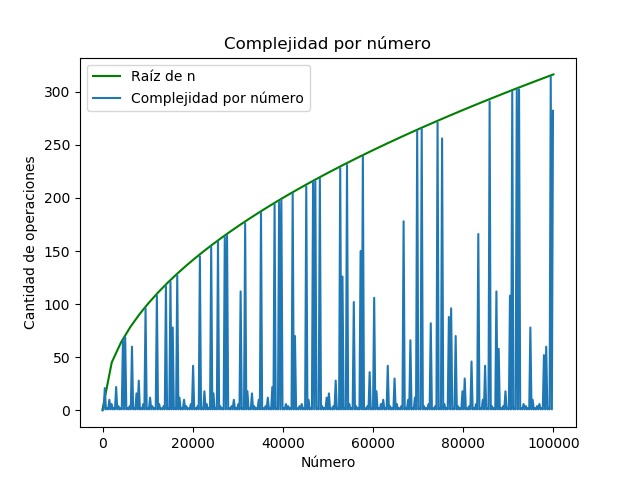
\includegraphics[scale=0.6]{Numeros1al100000.png}
\end{center}
En esta gr\'afica podemos observar que en algunos n\'umeros el algoritmo realiza una cantidad muy grande de operaciones, esto courre cuando los n\'umeros son primos pues el algoritmo tiene que verificar si el n\'umero es divisible por todos y cada uno de los numeros menores a la ra\'iz. Cuando el algoritmo realiza una menor cantidad de operaciones podemos inferir que se trata de n\'umeros impares no primos y/o n\'umeros pares los cuales necesitan la menor cantidad de operaciones debido a que el algoritmo verifica primero si los n\'umeros son divisibles entre 2.


\subsection{Segundo an\'alisis: N\'umeros del 1 al 50,000 y del 50,001 al 100,000}
\begin{center}
	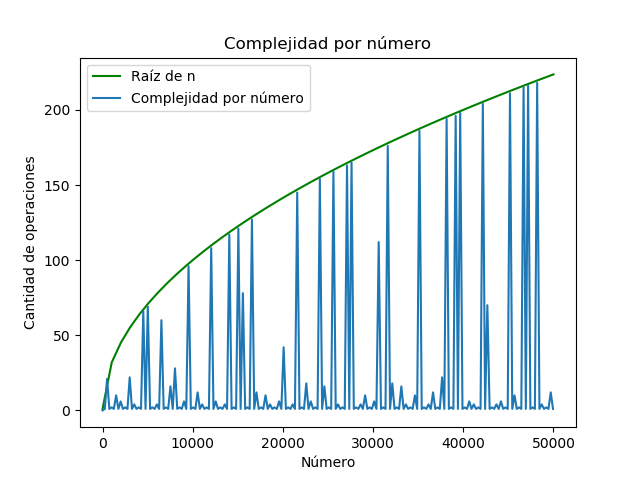
\includegraphics[scale=0.5]{Numeros1al50000.png}
    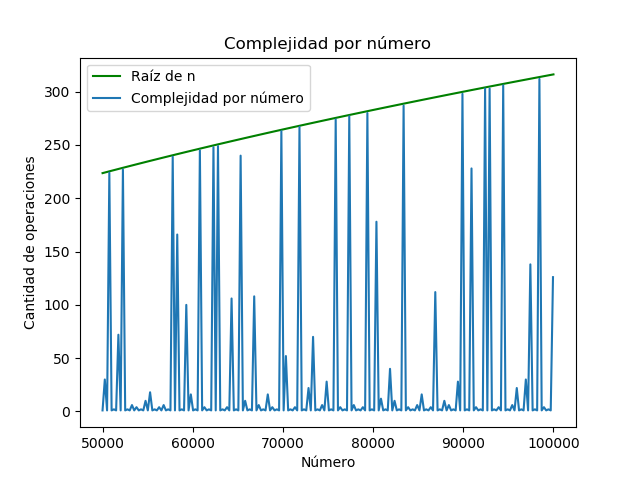
\includegraphics[scale=0.5]{Numeros50000al100000.png}
\end{center}
*Con estas dos gr\'aficas podemos tomar en cuenta varios factores:
\begin{itemize}
\item Se puede ver con mayor precisi\'on la distribuci\'on de los n\'umeros primos
\item Hay una mayor cantidad de primos en los primeros 50,000
\item La cantidad de operaciones que se realizan en los n\'umeros del 50,000 al 100,000 es mayo
\end{itemize}


\subsection{Tercer an\'alisis: N\'umeros pares}
\begin{center}
	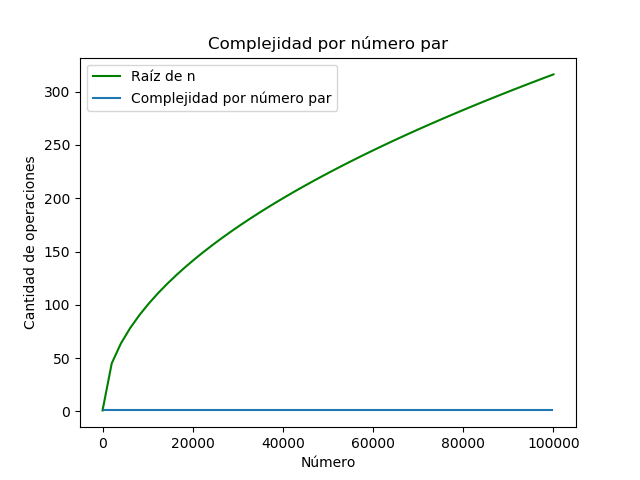
\includegraphics[scale=0.6]{NumerosPares.png}
\end{center}
En esta gr\'afica podemos observar como se dijo en el primer an\'alisis, el algoritmo realiza la cantidad m\'inima de operaciones debido a que primero se verifica si el n\'umero es divisible entre 2, condici\'on que cumple todo n\'umero par.


\subsection{Cuarto an\'alisis: N\'umeros impares}
\begin{center}
	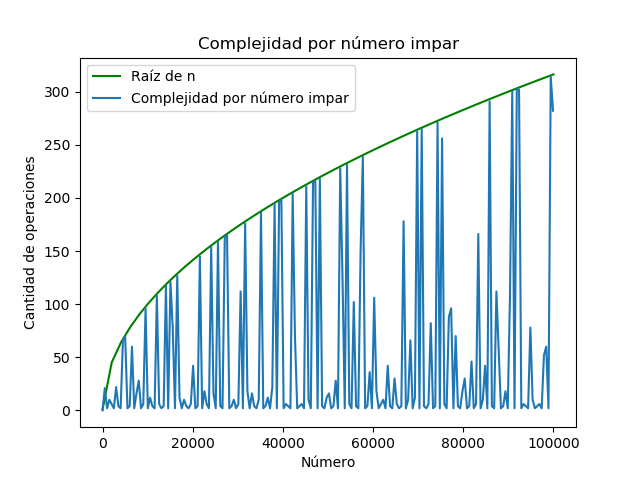
\includegraphics[scale=0.6]{NumerosImparesconPrimos.png}
\end{center}
Sabemos que los n\'umeros primos son impares y debido a eso en esta gr\'afica podemos observar que se realiza la mayor cantidad de operaciones en algunos n\'umeros. En los n\'umeros impares no primos se realiza una gran cantidad de operaciones, mayor a la de los n\'umeros pares y menor a la de los n\'umeros primos debido a que el algoritmo tarda m\'as en encontrar un divisor, sin embargo lo encuentra en menos de $\sqrt{n}$ operaciones.

\newpage \'Esta es la gr\'afica para los n\'umeros impares no primos, en la cual verificamos lo mencionado anteriormente.
\begin{center}
	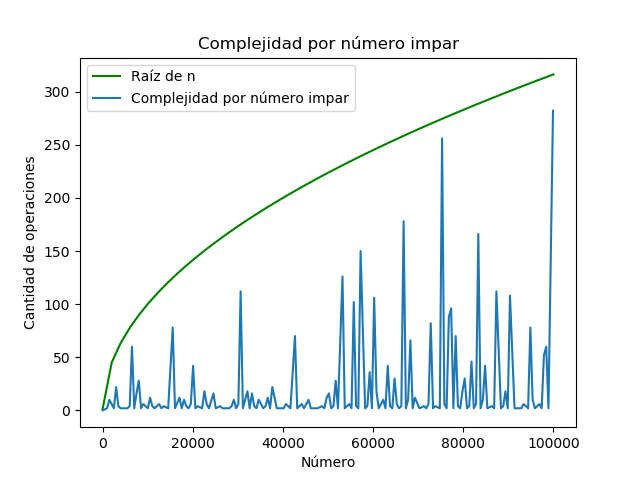
\includegraphics[scale=0.6]{NumerosImpares.png}
\end{center}



\subsection{Quinto an\'alisis: N\'umeros primos}
\begin{center}
	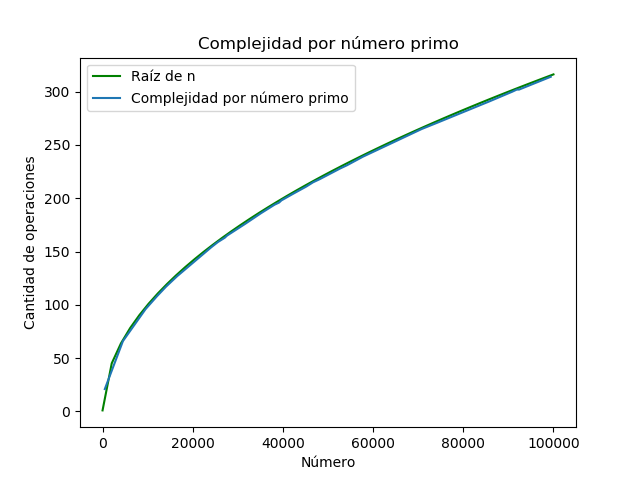
\includegraphics[scale=0.6]{NumerosPrimos.png}
\end{center}
En esta gr\'afica podemos observar que el algoritmo realiza la m\'axima cantidad de operaciones para cada n\'umero. El algoritmo realiza operaciones para verificar si el n\'umero es divisible entre alg\'un n\'umero menor a su ra\'iz, lo cual no sucede y ocasiona que el algoritmo visite cada uno de \'estos n\'umeros, por eso es que vemos que la curva que representa las operaciones realizadas esta tan cerca de la curva que representa la ra\'iz de cada n\'umero.

\section{Conclusiones}
*Se necesitan los an\'alisis completos para las conclusiones

\end{document}
